% This is a LaTeX thesis template for Adam Mickiewicz University.
% to be used with Rmarkdown
% This template was produced by Jakub Nowosad
% Version: 16 February 2020

% Inspired by:
% This is a LaTeX thesis template for Monash University.
% to be used with Rmarkdown
% This template was produced by Rob Hyndman
% Version: 6 September 2016

\documentclass{amuthesis}
% \usepackage[polish]{babel}
\usepackage{polski}
\renewcommand{\figurename}{Rycina} % Redefine default figure caption %
\renewcommand{\tablename}{Tabela} % Redefine default table caption %
%%%%%%%%%%%%%%%%%%%%%%%%%%%%%%%%%%%%%%%%%%%%%%%%%%%%%%%%%%%%%%%
% Add any LaTeX packages and other preamble here if required
%%%%%%%%%%%%%%%%%%%%%%%%%%%%%%%%%%%%%%%%%%%%%%%%%%%%%%%%%%%%%%%
\usepackage{booktabs,tabularx} % Allows kableExtra to work %
\usepackage{indentfirst} % Adds indent in the first paragraph %
\usepackage{bookmark} % Adds indent in the first paragraph %

\author{Błażej Kościański}
\title{Porównanie metod (miar?) określania zmian struktury przestrzennej
kategorii pokrycia terenu}
\def\titleeng{TODO}
\def\degreetitle{Praca magisterska}
\def\major{Geoinformacja}
\def\albumid{444861}
\def\thesisyear{2023}

% Add subject and keywords below
\hypersetup{
     %pdfsubject={The Subject},
     %pdfkeywords={Some Keywords},
     pdfauthor={Błażej Kościański},
     pdftitle={Porównanie metod (miar?) określania zmian struktury
przestrzennej kategorii pokrycia terenu},
     pdfproducer={quarto with LaTeX}
}

\bibliography{thesis.bibpackages.bib}

\begin{document}

\pagenumbering{arabic}

\titlepage

\bookmarksetup{startatroot}

\hypertarget{streszczenie}{%
\chapter*{Streszczenie}\label{streszczenie}}
\addcontentsline{toc}{chapter}{Streszczenie}

\markboth{Streszczenie}{Streszczenie}

\textbf{Abstrakt}

Streszczenie powinno przedstawiać skrótowo główny problem pracy i jego
rozwiązanie. Możliwa struktura streszczenia to: (1) 1-3 zdania wstępu do
problemu (czym się zajmujemy, dlaczego jest to ważne, jakie są
problemy/luki do wypełnienia), (2) 1 zdanie opisujące cel pracy, (3) 1-3
zdania przedstawiające użyte materiały (dane) i metody (techniki,
narzędzia), (4) 1-3 zdania obrazujące główne wyniki pracy, (5) 1-2
zdania podsumowujące; możliwe jest też określenie dalszych
kroków/planów.

Słowa kluczowe: (4-6 słów/zwrotów opisujących treść pracy, które nie
wystąpiły w tytule)

\textbf{Abstract}

The abstract must be consistent with the above text.

Keywords: (as stated before)

\newpage

\setstretch{1.2}\sf\tighttoc\doublespacing

\bookmarksetup{startatroot}

\hypertarget{sec-wprowadzenie}{%
\chapter{Wprowadzenie}\label{sec-wprowadzenie}}

Informacje geograficzne stanowią wyniki selekcji i przetwarzania danych
\textbf{dotyczących aspektów} otaczającej nas przestrzeni geograficznej.
Pozwalają na bardziej zrozumiałe i efektywne analizowanie, modelowanie
oraz interpretowanie złożonych zjawisk i procesów zachodzących w naszym
otoczeniu. Informacje geograficzne i ich aspekty nie stanowią
niepodważalnych faktów, lecz często powstają w wyniku działań jednostek,
jak i wspólnych wysiłków grup ekspertów, którzy zajmują się wyborem,
analizą i klasyfikacją danych geograficznych \autocite{WhatIsLandCover}.
W procesie tworzenia informacji geograficznych istnieje zatem pewien
stopień subiektywności, który może wpłynąć na ostateczny kształt
(ostateczną postać?) tych informacji, ich interpretację, jak i na ich
użyteczność w kontekście innych zastosowań. Przykładem informacji
geograficznej, której ostateczna postać zależna jest od założeń
przyjętych w trakcie tworzenia danych przestrzennych, jest pokrycie
terenu.

Przyjmuje się, że termin pokrycie terenu obejmuje zbiór wszelkich
elementów obecnych na powierzchni Ziemi (\textbf{dodać ref}). W elementy
pokrycia terenu włączają się obiekty związane z działalnością człowieka,
skutkami sił przyrody oraz wszelkie inne istniejące obiekty, które mogą
znaleźć się w przestrzeni geograficznej (\textbf{dodać ref}). Tworzenie
dokładnych i wiarygodnych danych dotyczących pokrycia terenu jest
niezbędne w kontekście wielu zastosowań, takich jak planowanie
przestrzenne (\textbf{dodać ref}), ochrona środowiska (\textbf{dodać
ref}), czy analiza zmian klimatycznych (\textbf{dodać ref}). Ostateczna
forma tych danych jest jednak w dużej mierze determinowana przez wybory
i założenia dokonywane w procesie ich tworzenia (\textbf{ewentualnie
dodać rycinę z przykładem mapy pokrycia terenu}). W tym kontekście,
analiza pokrycia terenu staje się istotnym polem badań, które skupia się
na zarówno na technicznych aspektach zbierania danych, jak i na ich
semantycznej interpretacji (\textbf{dodać ref}).

\textbf{w tym akapicie gdzieś wspomnieć o rastrach} Dane oraz wynikowe
mapy pokrycia terenu są rezultatem złożonego procesu przetwarzania i
analizy danych przestrzennych najczęściej w postaci obrazów
satelitarnych (\textbf{dodać ref}). Na początku tego procesu, satelity
wyposażone w sensory rejestrują obrazy Ziemi z różnych zakresów
widmowych. Uzyskane obrazy mogą być interpretowane manualnie przez grupy
specjalistów. Pozwala to na uzyskanie map pokrycia terenu o wysokiej
dokładności, kosztem długiego procesu ich tworzenia (\textbf{dodać
ref}). Dużo mniej czasochłonną metodą jest przetwarzanie przy użyciu
algorytmów. Umożliwiają one względnie szybką, półautomatyczną
identyfikację i klasyfikację różnych typów powierzchni kosztem mniejszej
dokładności mapy wynikowej (\textbf{dodać ref}). Ostatecznie, dane
przekształcone w mapy pokrycia terenu mogą posłużyć do analiz zmian
pokrycia terenu (\textbf{dodać ref}).

Celem analiz zmian pokrycia terenu jest przede wszystkim monitorowanie i
pogłębienie aktualnej wiedzy na temat ewolucji otaczającego nas
krajobrazu (\textbf{dodać ref}). Jest to istotne w kontekście ochrony
przyrody (\textbf{dodać ref}), planowania przestrzennego (\textbf{dodać
ref}), oceny wpływu inwestycji (\textbf{dodać ref}) i infrastruktury na
środowisko (\textbf{dodać ref}), a także w badaniach naukowych
dotyczących zmian klimatycznych (\textbf{dodać ref}), bioróżnorodności
(\textbf{dodać ref}) oraz innych procesów ekologicznych
\autocite{ChangeDetectionTechniques}. Dzięki analizie zmian pokrycia
terenu można identyfikować obszary zagrożone degradacją, monitorować
skutki urbanizacji, deforestacji czy erozji, co umożliwia podejmowanie
odpowiednich działań w celu zrównoważonego zarządzania środowiskiem i
zachowaniem jego integralności.

W badaniach nad zmianami pokrycia terenu wykorzystuje się różnorodne
metody analityczne. Niemniej jednak, wiele z tych technik koncentruje
się na analizie zmian na poziomie indywidualnych komórek w siatce rastra
\autocite{ChangeDetectionTechniques}. Choć podejście to może dostarczać
użytecznych informacji dotyczących trendów zmian pokrycia terenu na
niewielkich obszarach, charakteryzuje się ono istotnymi ograniczeniami w
kontekście interpretacji wyników. Szczególnie w przypadku badań
obejmujących rozległe terytoria, takie jak kraje czy nawet kontynenty,
bardziej efektywne staje się zastosowanie metod opartych na analizie
struktur przestrzennych \autocite{Netzel2015}. Głównym założeniem tych
metod jest przekształcenie danych z postaci pojedynczych wartości
komórek rastra w sygnatury przestrzenne, a następnie porównanie ich ze
sobą za pomocą miar odległości i niepodobieństwa.

Sygnatury przestrzenne stanowią statystyczny opis struktur
przestrzennych kategorii pokrycia terenu na mniejszych, wydzielonych
obszarach w obrębie całego zbioru danych. W celu porównania ze sobą
dwóch sygnatur przestrzennych, wykorzystywane są miary niepodobieństwa.
Umożliwiają one określenie w jakim stopniu dwa analizowane obszary się
od siebie różnią pod względem kompozycji oraz konfiguracji
przestrzennej. Opracowane zostało wiele różnych miar niepodobieństwa,
takich jak odległość euklidesowa, odległość Canberra, metryka Wave
Hedges, współczynnik podobieństwa Jaccarda, odległość Jensena-Shannona
czy dywergencja Pearsona \autocite{Cha2007}. Współcześnie jednak nie
określono, która z tych miar jest najbardziej zgodna zarówno z
postrzeganiem przez człowieka, jak i wpływem zmian na procesy
środowiskowe.

wady i zalety obu podejść, np. że percepcja jest subiektywna i nie
skaluje się

Celem tej pracy było porównanie metod określania zmian struktury
przestrzennej kategorii pokrycia terenu w kontekście ich korelacji z
postrzeganiem zmian przestrzennych przez ludzi. W celu realizacji tego
zadania przeprowadzone zostały ankiety, w których zadaniem respondentów
było określenie stopnia podobieństwa między parami rastrów. Badania
przeprowadzone zostały na rastrach składających się wyłącznie z dwóch
lub trzech kategorii. Wyniki ankiety zestawione zostały z wartościami 46
miar niepodobieństwa. Na tej podstawie, do dalszej analizy wybrane
zostało 8 miar niepodobieństwa charakteryzujących się największą
zgodnością z ludzką percepcją zmian przestrzennych.

\bookmarksetup{startatroot}

\hypertarget{sec-metody}{%
\chapter{Metody}\label{sec-metody}}

W tym rozdziale zostaną kolejno opisane wszystkie zagadnienia kluczowe
do zrozumienia tematyki określania zróżnicowania struktur przestrzennych
w kontekście zmian pokrycia terenu. W pierwszej kolejności wyjaśnione
zostanie zagadnienie struktur przestrzennych. Następnie omówione zostaną
wskaźniki umożliwiające określanie charakterystyk struktur
przestrzennych, czyli metryki krajobrazowe oraz sygnatury przestrzenne.
Omówione zostaną koncepcje kompozycji oraz konfiguracji przestrzennej, a
także miary umożliwiające ich obliczenie. Opisana zostanie także idea
reprezentacji rastrów w postaci macierzy i wektorów współwystępowania. W
następnej kolejności zostaną przedstawione dwie metody analiz zmian
pokrycia terenu. Pierwsza, opierająca się na analizie różnic na poziomie
indywidualnych komórek w siatce rastra, oraz druga, oparta na analizie
struktur przestrzennych występujących wewnątrz rastra. Wyjaśnione
zostaną zagadnienia miar odległości i niepodobieństwa oraz ich
wykorzystania w analizach przestrzennych. Przedstawiony zostanie także
proces obliczenia niepodobieństwa między parą rastrów. W końcowej części
rozdziału opisany zostanie sposób symulacji danych rastrowych o
określonej kompozycji i konfiguracji przestrzennej.

\hypertarget{struktury-przestrzenne}{%
\section{Struktury przestrzenne}\label{struktury-przestrzenne}}

Znaczna część dziedziny ekologii krajobrazu opiera się na paradygmacie
płatów \autocite{mcgarigal2009}. Według tej idei krajobrazy składają się
z jednostek (płatów), które charakteryzuje się jako wyodrębnione obszary
o jednakowej kategorii pokrycia terenu
\autocite{forman1995land,solon2002}. Każdy krajobraz natomiast cechuje
się pewną strukturą przestrzenną, której różne cechy mogą następnie być
opisywane na przykład za pomocą metryk krajobrazowych lub sygnatur
przestrzennych.

\hypertarget{metryki-krajobrazowe}{%
\section{Metryki krajobrazowe}\label{metryki-krajobrazowe}}

Metryki krajobrazowe umożliwiają analizę struktury przestrzennej
krajobrazu na podstawie danych o pokryciu terenu
\autocite{Pukowiec_Kurda_Sobala_2016}. Można je podzielić na dwie grupy:
wskaźniki kompozycji i konfiguracji
\autocite{solon2002,Pukowiec_Kurda_Sobala_2016}. Celem pierwszej grupy
metryk jest opis kompozycji (udziału) rastrów, czyli zróżnicowania i
liczby płatów poszczególnych kategorii pokrycia terenu bez uwzględniania
informacji o ich lokalizacji w przestrzeni
\autocite{Gustafson1998,solon2002,kozak2014}. Konfiguracja (ułożenie)
natomiast w sposób liczbowy opisuje sąsiadowanie ze sobą poszczególnych
płatów \autocite{Gustafson1998,solon2002,kozak2014}. Szczególną zaletą
takiego podejścia jest to, że metryki krajobrazowe mogą być obliczone
dla różnorodnych jednostek przestrzennych, które mogą być zdefiniowane
na podstawie wszelkich aspektów administracyjnych, geograficznych,
biogeograficznych lub umownych \autocite{Pukowiec_Kurda_Sobala_2016}.
Jednostki te mogą obejmować zarówno granice gmin, zlewni, ekoregionów
czy nawet abstrakcyjne obszary na mapie, co z kolei umożliwia
wszechstronne stosowanie tych metryk w badaniach związanych z analizą
krajobrazu.

\hypertarget{sygnatury-przestrzenne}{%
\section{Sygnatury przestrzenne}\label{sygnatury-przestrzenne}}

Często w celu lepszej reprezentacji analizowanych rastrów możemy
wykorzystywać także bardziej skomplikowane sygnatury przestrzenne.
Przykładem sygnatury łączącej zarówno kompozycję, jak i konfigurację
przestrzenną jest macierz współwystępowania. Jest to macierz o wymiarach
k na k, gdzie k reprezentuje liczbę kategorii pokrycia terenu obecnych w
analizowanym rastrze \autocite{Haralick_1973,Jasiewicz_GeoPAT}. Macierz
tą możemy skonstruować poprzez zliczanie kolejno wszystkich par
sąsiadujących ze sobą komórek w rastrze. Wewnątrz tej macierzy, wartości
ułożone na przekątnej odnoszą się do kompozycji rastra, natomiast
pozostałe do jego konfiguracji. Przykład dwóch macierzy
współwystępowania dla rastrów o zbliżonej kompozycji i różnej
konfiguracji przestrzennej przedstawia Rycina \ref{fig-metody-coma}.

\begin{figure}[t]

{\centering 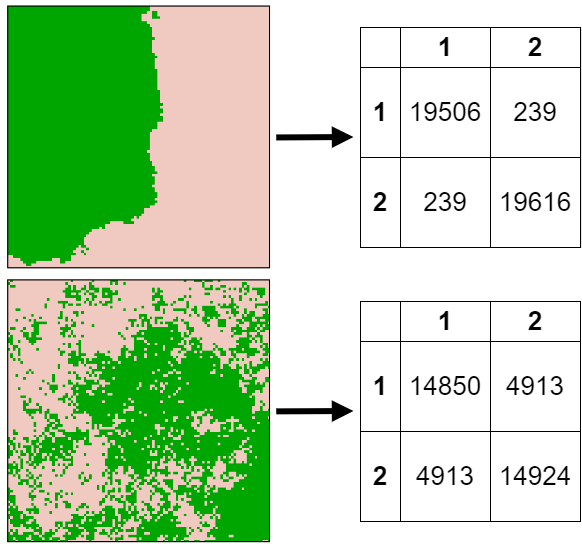
\includegraphics[width=3.64583in,height=3.64583in]{figures/diagram_coma.png}

}

\caption{\label{fig-metody-coma}Przykład dwóch macierzy
współwystępowania dla rastrów o zbliżonej kompozycji i różnej
konfiguracji przestrzennej.}

\end{figure}

Na podstawie macierzy współwystępowania mogą zostać obliczone różne
miary wywodzące się z dziedziny teorii informacji. Przykładem takiej
miary jest entropia brzegowa \textbf{\emph{PRZYKŁADY, JAK JEST LICZONA,
WZÓR}} która opisuje zróżnicowanie kompozycji rastra, czyli udziałów
każdej z kategorii w rastrze.

\[
H(y) = -\sum_{j=1}^{K}p(y=c_{j})log_2p(y=c_j)
\] \[
H(y|x) = \sum_{i=1}^{K}\sum_{j=1}^{K} p(x=c_i, y=c_j) log_2 p(y=c_i | x=c_j)
\]

\[
I(y,x) = H(y) - H(y|x)
\] \[
U = I(y,x)/H(y)
\]

Kolejną miarą jest względna informacja wzajemna \textbf{\emph{PRZYKŁADY,
JAK JEST LICZONA, WZÓR}}. Reprezentuje ona stopień sąsiadowania ze sobą
kategorii w rastrze, czyli jego konfigurację przestrzenną. W celu
porównywania ze sobą sygnatur dwóch rastrów w postaci dwuwymiarowej
macierzy należy je sprowadzić do postaci jednowymiarowego wektora, a
następnie przeprowadzić jego normalizację, tak aby wszystkie wartości
sumowały się do 1. Taka postać pozwala na obliczanie miar odległości lub
podobieństwa, pozwalających na porównywanie histogramów wartości
\autocite{Cha2007}. Miary te następnie pozwalają określić stopień
odmienności dwóch rastrów. Podejście to może być także wykorzystane w
innych analizach przestrzennych, jak wyszukiwanie obszarów o podobnej
strukturze przestrzennej, wykrywanie ich zmian oraz grupowanie obszarów
o podobnej strukturze przestrzennej
\autocite{Jasiewicz_GeoPAT,nowosad_motif}.

\hypertarget{metody-analiz-ruxf3ux17cnic-pokrycia-terenu}{%
\section{Metody analiz różnic pokrycia
terenu}\label{metody-analiz-ruxf3ux17cnic-pokrycia-terenu}}

Różnice w pokryciu terenu można analizować przy użyciu różnych metod.
Wiele z nich koncentruje się na analizie różnic na poziomie
indywidualnych komórek w siatce rastra. Najbardziej podstawowym
przykładem takiego podejścia jest analiza ilościowa różnic w pokryciu
terenu. Zaletą tego podejścia jest przede wszystkim łatwość w wykonaniu
analizy. Wystarczy zliczyć wszystkie komórki należące do poszczególnych
kategorii dla wybranych rastrów, a następnie porównać ze sobą te
wartości, aby otrzymać wynik informujący nas o ilościowych różnicach
między analizowanymi rastrami. Analiza ilościowa najczęściej
wykorzystywana jest w celu wskazania ogólnych trendów zmian pokrycia
terenu dla określonego obszaru badań jak na przykład zmniejszanie się
obszarów leśnych lub wzrost terenów zurbanizowanych.

Wszelkie metody analiz zmian pokrycia terenu opierające się na analizie
poszczególnych komórek w siatce rastra są użyteczne na obszarach, gdzie
zmiany między indywidualnymi komórkami dostarczają istotnych informacji.
Ich przydatność jednak maleje, gdy informacja na poziomie pojedynczej
komórki przestaje być tak istotna, na przykład dla rastrów o wysokiej
rozdzielczości lub znacznym zasięgu przestrzennym
\autocite{Jasiewicz_GeoPAT}. W takiej sytuacji bardziej efektywne staje
się zastosowanie metod opartych na analizie struktur przestrzennych
\autocite{Netzel2015}.

Metody oparte na analizie struktur przestrzennych wywodzą się z
dziedziny ekologii krajobrazu. Pozwalają one przede wszystkim na opis
oraz obliczenie podobieństwa struktur przestrzennych. Głównym zamysłem
tych metod jest przekształcenie danych z postaci dużych rastrów
zbudowanych z wielu indywidualnych komórek zawierających pojedyncze
informacje w sygnatury przestrzenne, a następnie porównanie ich za
pomocą miar odległości lub niepodobieństwa. Sygnatura przestrzenna
stanowi statystyczny opis pewnych struktur przestrzennych występujących
wewnątrz rastra \autocite{Jasiewicz_GeoPAT,nowosad_motif}. Dokładnie w
tym samym celu wykorzystywane są także metryki krajobrazowe. Mają one
jednak istotną wadę w kontekście kompleksowych analiz przestrzennych.
Jako że pojedyncza metryka krajobrazowa reprezentuje wyłącznie jedną,
konkretną charakterystykę analizowanego obszaru, to nie jest w stanie
zdefiniować całej charakterystyki przestrzennej danego rastra. W tym
celu bardziej efektywne może być zastosowanie sygnatur przestrzennych.
Są one dwuwymiarową reprezentacją kompozycji i konfiguracji
przestrzennej rastra, czyli jego najbardziej podstawowych
charakterystyk. Oznacza to też, że można je ze sobą porównywać przy
użyciu szerokiej gamy istniejących miar odległości i niepodobieństwa.
Umożliwia to także wykonywanie bardziej skomplikowanych analiz
przestrzennych, jak wyszukiwanie, wykrywanie zmian, grupowanie i
segmentacja \autocite{nowosad_motif}.

\hypertarget{miary-odlegux142oux15bci-i-niepodobieux144stwa}{%
\section{Miary odległości i
niepodobieństwa}\label{miary-odlegux142oux15bci-i-niepodobieux144stwa}}

Odległość i rozbieżność (inaczej niepodobieństwo) stanowią pewien
policzalny stopień zróżnicowania pary obiektów. Największą różnicą
między nimi jest to, że odległości są symetryczne, podczas gdy
rozbieżności są niesymetryczne. Oznacza to, że wyłącznie dla miar
odległości otrzymujemy identyczny wynik przy porównywaniu par obiektów A
i B, jak i par B i A.

Niepodobieństwo jest przeciwieństwem podobieństwa. Ponadto, miary
podobieństwa można łatwo przekształcić w miary niepodobieństwa
\autocite{niesterowicz2016}. W związku z tym, w celu uproszczenia
terminologii, wszystkie miary odległości, podobieństwa oraz te wywodzące
się z dziedziny teorii informacji, które zostały wykorzystane w tej
pracy, będą dalej zbiorowo nazywane miarami niepodobieństwa.

Wybór odpowiedniej miary niepodobieństwa zależy między innymi od rodzaju
pomiaru lub sposobu reprezentacji obiektów \autocite{Cha2007}. Na
podstawie podobieństw syntaktycznych, wyróżnia się kilka grup rodzin
miar niepodobieństwa \autocite{Cha2007}: rodzina Minkowski (odległość
euklidesowa, odległość Minkowskiego, odległość Manhattan), rodzina L1
(Canberra, Sorensen, Kulczynski), rodzina Intersection (Intersection,
Wave Hedges, Ruzicka), rodzina Inner Product (Jaccard, Harmonic mean),
rodzina Squared-chord (Fidelity, Matusita), rodzina Squared L2 (Clark,
Pearson X2, Neyman X2), rodzina Shannon's Entropy (Jensen-Shannon,
Kullback-Leibler), a także miary będące połączeniem innych miar (Taneja,
Kumar-Johnson) oraz miary wywodzące się z teorii informacji (informacja
wzajemna, entropia Shannona).

\hypertarget{przykux142ad-obliczenia-niepodobieux144stwa-rastruxf3w}{%
\section{Przykład obliczenia niepodobieństwa
rastrów}\label{przykux142ad-obliczenia-niepodobieux144stwa-rastruxf3w}}

Pierwszym krokiem, jaki należy podjąć w celu obliczenia podobieństwa
struktur przestrzennych danych rastrowych z wykorzystaniem metod
opartych o sygnatury przestrzenne jest sprowadzenie rastrów wejściowych
do postaci macierzy współwystępowania. Proces utworzenia macierzy
współwystępowania polega na zliczeniu wartości każdej indywidualnej
komórki rastra, a także przylegających do niej komórek (najczęściej
czterech lub ośmiu). Przykładowe macierze współwystępowania widoczne są
na Rycinie \ref{fig-metody-coma}. Następnie, dwuwymiarową macierz należy
sprowadzić do postaci jednowymiarowej, czyli wektora współwystępowania.
Kolejnym etapem analizy jest normalizacja wektora współwystępowania. Po
dodaniu do siebie wszystkich wartości tego wektora powinniśmy otrzymać
wynik równy 1. Po wykonaniu powyższych czynności otrzymujemy
reprezentację rastrów wejściowych, która umożliwia porównanie ich ze
sobą przy użyciu miar niepodobieństwa między rozkładami
prawdopodobieństwa, takich jak rozbieżnosć Jensena-Shannona. Proces
obliczenia niepodobieństwa dwóch rastrów w postaci schematu przedstawia
Rycina \ref{fig-schemat-porownanie}.

\begin{figure}[t]

{\centering 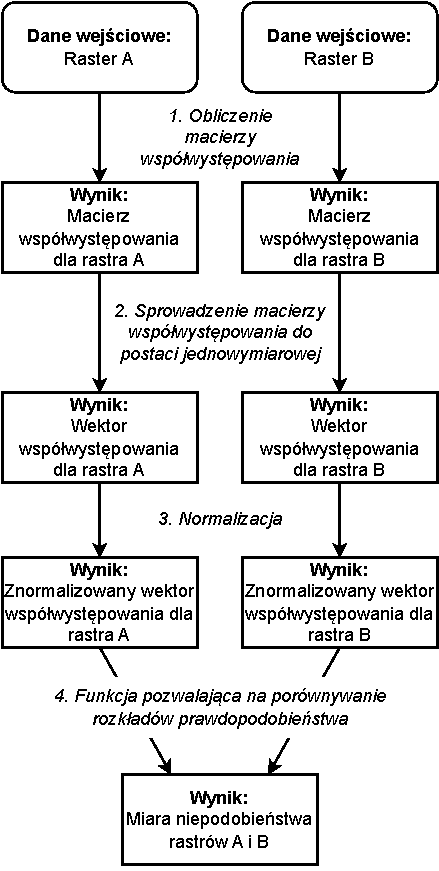
\includegraphics[width=3.125in,height=6.25in]{figures/diagram_raster_comparison.pdf}

}

\caption{\label{fig-schemat-porownanie}Schemat procesu obliczenia
niepodobieństwa dwóch rastrów.}

\end{figure}

\hypertarget{symulowanie-rastruxf3w-o-okreux15blonej-kompozycji-i-konfiguracji-przestrzennej}{%
\section{Symulowanie rastrów o określonej kompozycji i konfiguracji
przestrzennej}\label{symulowanie-rastruxf3w-o-okreux15blonej-kompozycji-i-konfiguracji-przestrzennej}}

Najważniejszym założeniem przy tworzeniu zbioru rastrów do pierwszej
ankiety było przygotowanie ich w sposób umożliwiający uzyskanie pełnej
reprezentacji wszystkich możliwych wartości kompozycji, jak i
konfiguracji przestrzennej. Zbiór rastrów został przygotowany w języku
programowania R \autocite{R2023}, w oparciu o wykorzystanie funkcji
\emph{nlm\_fbm} z pakietu NLMR \autocite{NLMR2018}. Funkcja ta pozwala
na symulację rastrów przy użyciu ułamkowych ruchów Browna, będących
uproszczeniem ruchów Browna \autocite{nlm_fbm}. W tej funkcji poziom
korelacji między kolejnymi krokami jest kontrolowany za pomocą parametru
``fract\_dim''. W kontekście tego badania, parametr ten reguluje
konfigurację przestrzenną. Oznacza to, że w przypadku, gdy
``fract\_dim'' przyjmuje niską wartość, wartości w generowanym rastrze
rozmieszczone są w sposób losowy, zbliżony do szumu. Natomiast w
przypadku wysokiej wartości ``fract\_dim'', na wynikowym rastrze tworzą
się skupiska najwyższych i najniższych wartości, a przejścia pomiędzy
nimi mają płynny, wygładzony charakter. Powyższa funkcja umożliwia
uzyskanie danych rastrowych wypełnionych wartościami
zmiennoprzecinkowymi mieszczącymi się w zakresie od 0 do 1 oraz
dowolnymi parametrami konfiguracji przestrzennej.

\begin{Shaded}
\begin{Highlighting}[]
\FunctionTok{library}\NormalTok{(RandomFields)}
\FunctionTok{library}\NormalTok{(NLMR)}

\NormalTok{sim1 }\OtherTok{=} \FunctionTok{nlm\_fbm}\NormalTok{(}\DecValTok{100}\NormalTok{, }\DecValTok{100}\NormalTok{, }\AttributeTok{fract\_dim =} \FloatTok{0.3}\NormalTok{)}
\NormalTok{sim2 }\OtherTok{=} \FunctionTok{nlm\_fbm}\NormalTok{(}\DecValTok{100}\NormalTok{, }\DecValTok{100}\NormalTok{, }\AttributeTok{fract\_dim =} \FloatTok{1.6}\NormalTok{)}

\NormalTok{sim\_stack1 }\OtherTok{=}\NormalTok{ raster}\SpecialCharTok{::}\FunctionTok{stack}\NormalTok{(sim1, sim2)}
\FunctionTok{names}\NormalTok{(sim\_stack1) }\OtherTok{=} \FunctionTok{c}\NormalTok{(}\StringTok{"wysokie fract\_dim"}\NormalTok{, }\StringTok{"niskie fract\_dim"}\NormalTok{)}

\FunctionTok{plot}\NormalTok{(sim\_stack1)}
\end{Highlighting}
\end{Shaded}

\begin{figure}[t]

{\centering \includegraphics{02-roz2_files/figure-pdf/unnamed-chunk-3-1.pdf}

}

\end{figure}

Następnie, aby otrzymać zbiór rastrów uwzględniający także pełen
przekrój kompozycji należy przeprowadzić proces reklasyfikacji.
Procedura ta polega na podziale każdego dotychczas utworzonego rastra na
kategorie pokrycia terenu w różnych proporcjach, na przykład 90:10,
70:30 oraz 50:50 w przypadku rastrów zawierających wyłącznie dwie
kategorie pokrycia terenu. Wykonanie tego procesu ułatwia między innymi
funkcja \emph{util\_binarize} z pakietu landscapetools
\autocite{NLMR2018}. W tej funkcji proporcje kategorii pokrycia terenu
kontrolowane są za pomocą parametru ``breaks''. Przykładowo, ustawienie
parametru ``breaks'' na poziomie \emph{0.2} poskutkuje otrzymaniem
rastra o kategoriach pokrycia terenu w proporcjach 20 do 80. Oznacza to,
że jedna z kategorii będzie obejmowała swoim zasięgiem 20\% komórek
rastra, podczas gdy druga kategoria wypełni pozostałe 80\% komórek.

\begin{Shaded}
\begin{Highlighting}[]
\FunctionTok{library}\NormalTok{(landscapetools)}

\NormalTok{sim1\_1 }\OtherTok{=}\NormalTok{ landscapetools}\SpecialCharTok{::}\FunctionTok{util\_binarize}\NormalTok{(sim1, }\AttributeTok{breaks =} \FloatTok{0.1}\NormalTok{)}
\NormalTok{sim1\_2 }\OtherTok{=}\NormalTok{ landscapetools}\SpecialCharTok{::}\FunctionTok{util\_binarize}\NormalTok{(sim1, }\AttributeTok{breaks =} \FloatTok{0.5}\NormalTok{)}

\NormalTok{sim2\_1 }\OtherTok{=}\NormalTok{ landscapetools}\SpecialCharTok{::}\FunctionTok{util\_binarize}\NormalTok{(sim2, }\AttributeTok{breaks =} \FloatTok{0.1}\NormalTok{)}
\NormalTok{sim2\_2 }\OtherTok{=}\NormalTok{ landscapetools}\SpecialCharTok{::}\FunctionTok{util\_binarize}\NormalTok{(sim2, }\AttributeTok{breaks =} \FloatTok{0.5}\NormalTok{)}

\NormalTok{sim\_stack2 }\OtherTok{=}\NormalTok{ raster}\SpecialCharTok{::}\FunctionTok{stack}\NormalTok{(sim1, sim1\_1, sim1\_2,}
\NormalTok{                           sim2, sim2\_1, sim2\_2)}

\FunctionTok{plot}\NormalTok{(sim\_stack2)}
\end{Highlighting}
\end{Shaded}

\begin{figure}[t]

{\centering \includegraphics{02-roz2_files/figure-pdf/unnamed-chunk-4-1.pdf}

}

\end{figure}

\begin{Shaded}
\begin{Highlighting}[]
\CommentTok{\# library(rasterVis)}
\CommentTok{\# gplot(sim\_stack2) + }
\CommentTok{\#   geom\_tile(aes(fill = value)) +}
\CommentTok{\#   facet\_wrap(\textasciitilde{} variable) +}
\CommentTok{\#   scale\_fill\_gradientn(colours = rev(terrain.colors(225))) +}
\CommentTok{\#   coord\_equal()}
\CommentTok{\# }
\CommentTok{\# \# wizualizacja symulowanych rastrów}
\CommentTok{\# tm\_shape(sim\_stack2) +}
\CommentTok{\#   tm\_raster(style = \textquotesingle{}cont\textquotesingle{}, breaks = c(0,2), palette = terrain.colors(255)) +}
\CommentTok{\#   tm\_layout(asp = 1, legend.show = FALSE, panel.show = FALSE)}
\end{Highlighting}
\end{Shaded}

\bookmarksetup{startatroot}

\hypertarget{sec-materialy}{%
\chapter{Materiały}\label{sec-materialy}}

W tym rozdziale zostanie omówiony cel przeprowadzenia pierwszej ankiety
oraz istotne aspekty związane z jej formą. Następnie opisany zostanie
sposób przygotowania danych wraz z przyjętą metodą doboru pytań do
ankiety.

\hypertarget{sec-przygotowanie1}{%
\section{Przygotowanie pierwszej ankiety}\label{sec-przygotowanie1}}

Najważniejszym założeniem przy tworzeniu zbioru rastrów do pierwszej
ankiety było przygotowanie ich w sposób umożliwiający uzyskanie pełnej
reprezentacji wszystkich możliwych wartości kompozycji, jak i
przestrzennej konfiguracji. Zbiór rastrów został przygotowany w oparciu
o wykorzystanie funkcji \emph{nlm\_fbm} z pakietu NLMR
\autocite{NLMR2018}. Funkcja ta pozwala na symulację rastrów przy użyciu
ułamkowych ruchów Browna, będących uproszczeniem ruchów Browna
\autocite{nlm_fbm}. W tej funkcji poziom korelacji między kolejnymi
krokami jest kontrolowany za pomocą parametru ``frac\_dim''. W
kontekście tego badania, parametr ten reguluje konfigurację
przestrzenną. Oznacza to, że w przypadku, gdy ``frac\_dim'' przyjmuje
niską wartość, wartości w generowanym rastrze rozmieszczone są w sposób
losowy, zbliżony do szumu. Natomiast w przypadku wysokiej wartości
``frac\_dim'', na wynikowym rastrze tworzą się skupiska najwyższych i
najniższych wartości, a przejścia pomiędzy nimi mają płynny, wygładzony
charakter. \textbf{\emph{tutaj dodać kawałek kodu pokazujący jak działa
funkcja?}} Kolejnym krokiem w procesie tworzenia danych było dodanie
zróżnicowania rastrów na podstawie ich przestrzennej kompozycji. Zostało
to osiągnięte poprzez podział każdego z wynikowych rastrów na kategorie
w oparciu o stałe przedziały wartości dla wszystkich rastrów. Proces

\begin{figure}[t]

{\centering 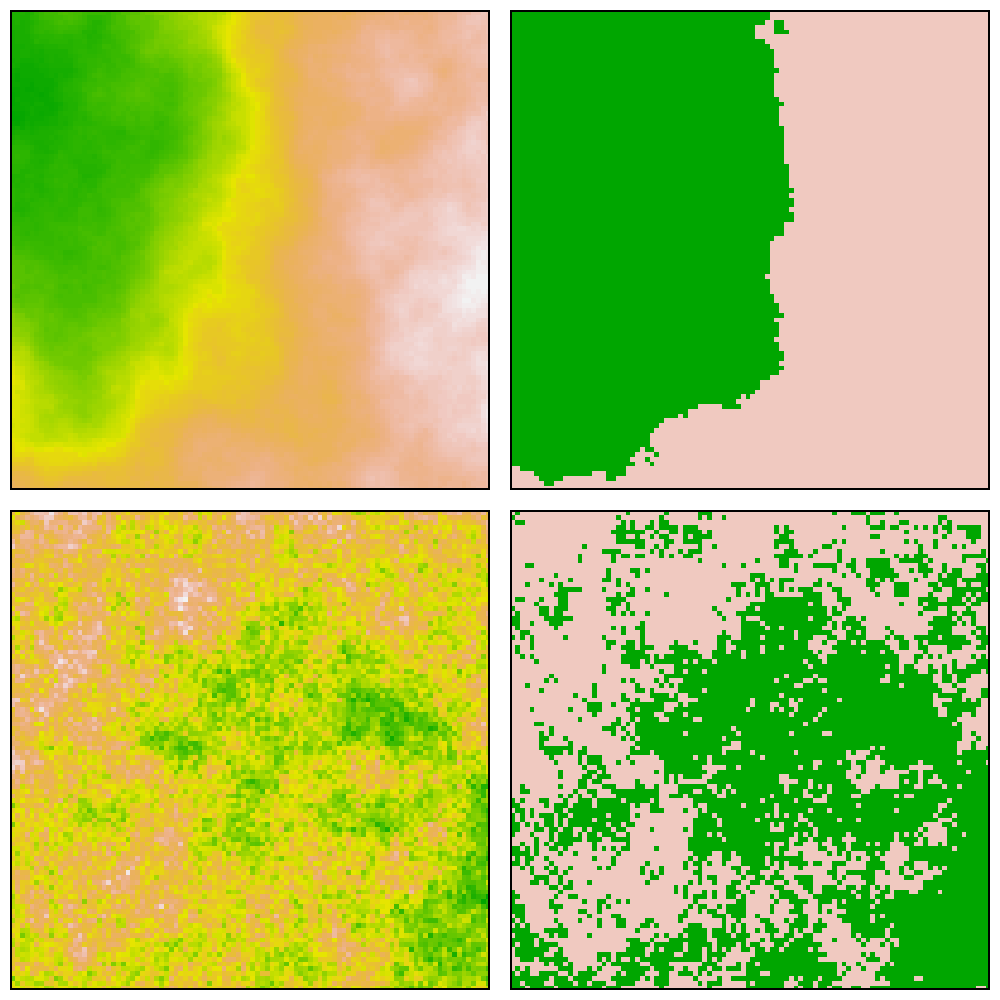
\includegraphics[width=4.16667in,height=4.16667in]{figures/wykres2_gen.png}

}

\caption{\label{fig-wykres2_gen}Wizualizacja procesu symulacji rastrów
do pierwszej ankiety albo placeholder zamiast pokazania jak działa
funkcja}

\end{figure}

W następnym etapie przygotowania danych obliczone zostały wybrane miary
opisujące struktury przestrzenne: entropia (ent) oraz względna
informacja wzajemna (relmutinf). Miary te umożliwiły potwierdzenie
uzyskania oczekiwanego rozkładu kompozycji i konfiguracji wewnątrz
zbioru rastrów.

Ostatecznie wygenerowane zostały zbiory rastrów składających się
wyłącznie z dwóch lub trzech kategorii pokrycia terenu. Przykład jednego
ze zbiorów rastrów przedstawia Rycina \ref{fig-wykres1_2classes}. Rastry
zawierające trzy kategorie zostały uwzględnione w badaniu w celu próby
wskazania czy liczba kategorii na rastrach ma wpływ na odpowiedzi
udzielane przez ankietowanych.

Ostatnim krokiem przygotowania danych było wybranie par rastrów
tworzących poszczególne pytania. W tym celu, pytania w ankietach
podzielone zostały na dwie grupy, wewnątrz których znalazły się po trzy
podgrupy pytań. W pierwszej kolejności respondenci zetknęli się z 24
pytaniami dotyczącymi rastrów uwzględniających wyłącznie dwie kategorie
pokrycia terenu, a następnie z 24 pytaniami uwzględniającymi trzy
kategorie pokrycia terenu. Pierwsza podgrupa pytań (6 par rastrów)
składała się z par rastrów różniących się między sobą wyłącznie
entropią. Podgrupa druga (6 par rastrów) zawierała wyłącznie rastry
różniące się względną informacją wzajemną. Ostatnia podgrupa (12 par
rastrów) składała się z pytań zróżnicowanych zarówno pod względem
entropii, jak i względnej informacji wzajemnej. Taki sposób doboru pytań
pozwolił na zredukowanie liczby odpowiedzi wymaganych od respondentów,
jak i ograniczenie wpływu błędu selekcji, który powstałby w wyniku
niewłaściwego doboru pytań. Respondenci celowo nie zostali poinformowani
o występujących różnicach pomiędzy kolejnymi pytaniami, ponieważ mogłoby
mieć to wpływ na udzielane przez nich odpowiedzi, co z kolei mogłoby
wpłynąć na ostateczne wyniki badania.

\begin{figure}[t]

{\centering 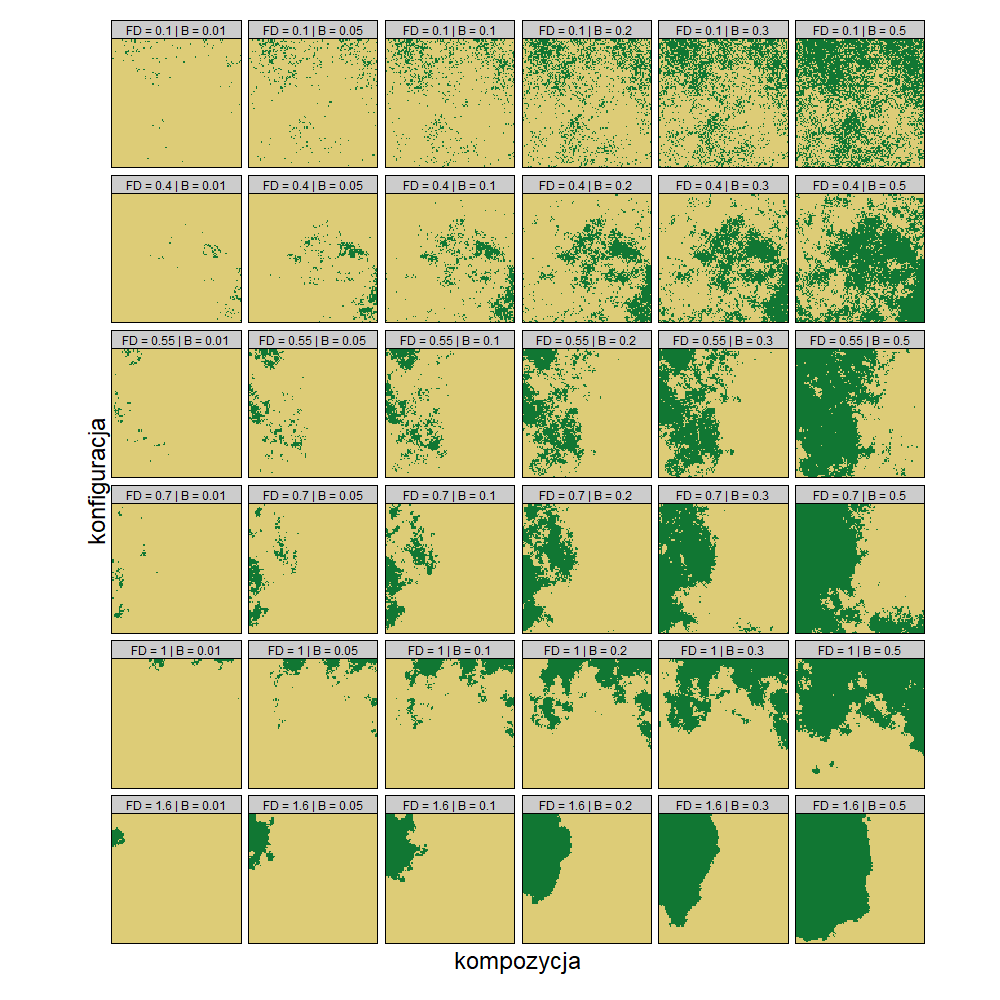
\includegraphics[width=1\textwidth,height=5.20833in]{figures/wykres1_2classes.png}

}

\caption{\label{fig-wykres1_2classes}Przykład zbioru wygenerowanych
rastrów (2 kategorie pokrycia terenu)}

\end{figure}

\hypertarget{sec-przygotowanie2}{%
\section{Przygotowanie drugiej ankiety}\label{sec-przygotowanie2}}

\hypertarget{sec-app}{%
\section{Ankieta w formie aplikacji shiny???}\label{sec-app}}

\bookmarksetup{startatroot}

\hypertarget{sec-wyniki}{%
\chapter{Wyniki}\label{sec-wyniki}}

W tym rozdziale przeprowadzona zostanie analiza i podsumowanie wyników
uzyskanych z ankiet. Wyniki zostaną zestawione z miarami niepodobieństwa
uwzględnionymi w analizie.

\hypertarget{sec-wyniki1}{%
\section{Wyniki pierwszej ankiety}\label{sec-wyniki1}}

Pierwsza ankieta została przeprowadzona w celu uzyskania wstępnych
informacji, mających na celu zrozumienie wpływu różnic w entropii oraz
względnej informacji wzajemnej między parami analizowanych rastrów na
wizualne postrzeganie zmian pokrycia terenu przez ludzi. Głównym celem
badania było wykazanie potencjalnych związków między percepcją zmian w
pokryciu terenu przez ludzi a miarami niepodobieństwa, które te zmiany
kwantyfikują. Przeprowadzenie ankiety pozwoliło także na wyznaczenie
dalszego kierunku badań, które miałyby zostać zrealizowane w kolejnej
ankiecie Section~\ref{sec-wyniki2}.

Badanie zostało realizowane w terminie od 21 do 24 listopada 2022 roku.
Proces zbierania odpowiedzi respondentów przyjął formę ankiety online,
co pozwoliło respondentom na wygodny udział w badaniu przy użyciu
komputera lub urządzenia mobilnego. Ankieta stworzona została w formie
aplikacji internetowej za pomocą języka programowania R, na podstawie
pakietów \textbf{shiny} \autocite*{R-shiny} oraz \textbf{shinysurveys}
\autocite*{R-shinysurveys} \textbf{\emph{NAPRAWIĆ BO NIE POKAZUJE SIĘ
CYTOWANIE W BIBLIOGRAFII}}. Sama aplikacja umieszczona została na
platformie shinyapps.io. Przeprowadzenie ankiety w formie online
umożliwiło systematyczne gromadzenie oraz przechowywanie odpowiedzi w
formie tabelarycznej, ułatwiając tym samym dalszą analizę i
interpretację danych. Respondenci stanowili grupę 50 studentów drugiego
roku studiów inżynierskich na kierunku Geoinformacja na Wydziale Nauk
Geograficznych i Geologicznych Uniwersytetu im. Adama Mickiewicza. Wybór
tej grupy respondentów oznacza, że byli oni już zaznajomieni z tematyką
tworzenia i analiz map w formie rastrowej oraz pojęciem zmian pokrycia
terenu.

Każdy z ankietowanych otrzymał do wypełnienia jeden z dwóch wcześniej
przygotowanych zbiorów pytań. Każdy ze zbiorów składał się z 48 pytań,
przy czym część pytań między zbiorami się pokrywała. Oznacza to, że
łącznie uzyskano odpowiedzi na 93 unikatowe pytania. W każdym z pytań
zadaniem respondentów było określenie podobieństwa na podstawie dwóch
załączonych rastrów. W ramach badania respondenci mieli możliwość
wyrażania swoich odpowiedzi za pomocą pięciostopniowej skali Likerta
\autocite{likert_scale}, która obejmowała poziomy od ``Brak'' przez
``Bardzo małe'', ``Umiarkowane'', ``Bardzo duże'' aż po ``Pełne''.
Wykorzystanie skali Likerta o nieparzystej liczbie przedziałów,
pozwoliło na zastosowanie przedziału środkowego, którego celem było
reprezentowanie odpowiedzi neutralnych lub trudnych do określenia.
Początkowo, zamiast skali Likerta planowano wykorzystać skalę liczbową,
w zakresie mieszczącym się od 1 do 100, jednakże zrezygnowano z tego
pomysłu, jako że znaczenie wartości na skali liczbowej może być
interpretowane inaczej przez każdego respondenta oraz skala ta nie
pozwala na uwzględnienie wspomnianej wcześniej odpowiedzi neutralnej.
Przykład pytania przedstawionego respondentom ilustruje Rycina
\ref{fig-przyklad_pytania}.

\begin{figure}[t]

{\centering 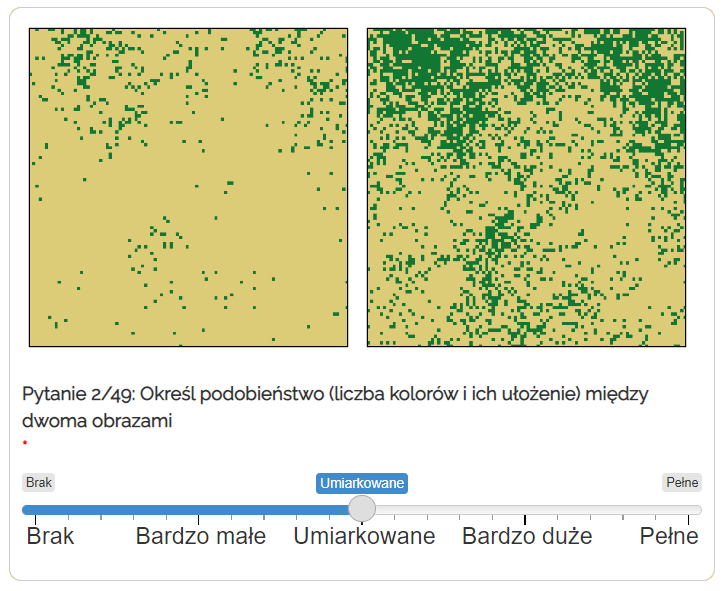
\includegraphics[width=1\textwidth,height=4.6875in]{figures/przyklad_pytania.png}

}

\caption{\label{fig-przyklad_pytania}Przykładowe pytanie z pierwszej
ankiety}

\end{figure}

Łącznie uzyskane zostało 2400 odpowiedzi na pytania z ankiety.
Podsumowanie uzyskanych odpowiedzi przedstawione zostało w Tabeli 1.

Według ankietowanych prawie 36\% par rastrów charakteryzowała się
brakiem podobieństwa, 32,6\% uzyskanych odpowiedzi wskazywało na bardzo
małe podobieństwo, 18,1\% na umiarkowane, 11,6\% bardzo duże, natomiast
mniej niż 2\% wskazywało na pełne podobieństwo. Warto tutaj także
zwrócić uwagę, że zestawienia wszystkich odpowiedzi w zależności od
liczby kategorii widocznych na rastrach nie wskazują na znaczące różnice
w liczbie odpowiedzi dla danej kategorii. Największą różnicę stanowi w
tym przypadku kategoria ``Bardzo duże'', dla której liczba odpowiedzi
dla rastrów z dwoma i trzema kategoriami pokrycia terenu różni się
zaledwie o 2,7\%. Najmniejszą różnicą charakteryzuje się kategoria
``Pełne'', gdzie liczba odpowiedzi pomiędzy zestawami różni się o jedyne
0,9\%.

Poziom zgodności każdego pytania został obliczony jako stosunek
najczęściej udzielonej odpowiedzi względem całkowitej liczby odpowiedzi.
Całkowity poziom zgodności ankietowanych został oszacowany na 55\%.
Oznacza to, że 1321 z 2400 udzielonych odpowiedzi znajdowało się w
grupie najczęstszej odpowiedzi dla danego pytania.

Pytania różniące się zarówno entropią, jak i względną informacją
wzajemną cechowały się najwyższym poziomem zgodności odpowiedzi
wynoszącym 61\%, podczas gdy pytania różniące się wyłącznie entropią
uzyskały wynik 53\%, a pytania różniące się wyłącznie względną
informacją wzajemną uzyskały wynik 52\%. Najwyższy poziom zgodności
odpowiedzi osób ankietowanych wyniósł 92\% i dotyczył pytania różniącego
się zarówno entropią, jak i względną informacją wzajemną (dopisać jak
bardzo różniły się ent i rmi). Najniższy poziom zgodności, czyli
zaledwie 38\%, osiągnęło aż 8 pytań. Wyłącznie dwa z nich dotyczyły
pytań zawierających trzy kategorie pokrycia terenu, podczas gdy
pozostałe - dwóch. 75\% z tych pytań uwzględniało rastry różniące się
pod względem względnej informacji przestrzennej (inna konfiguracja) przy
zachowaniu tej samej entropii (identyczna kompozycja).

W dalszym etapie analizy wyniki uzyskane z przeprowadzonej ankiety
zostały zestawione z wynikami 45 różnych miar niepodobieństwa dla par
rastrów uwzględnionych w ankiecie. Aby ocenić relacje między
najczęstszymi odpowiedziami uczestników ankiety a miarami
niepodobieństwa, przeprowadzono analizę korelacji Spearmana. W ten
sposób uzyskano ostateczny ranking miar, który został przedstawiony w
Tabeli 1.

Na podstawie analizy korelacji można wywnioskować, że spośród 45
uwzględnionych w badaniu metod obliczania podobieństwa między parami
rastrów, jedynie 6 z nich wykazuje dodatnią korelację z wynikami
uzyskanymi z ankiety. Spośród wszystkich metod, najwyższą wartość
korelacji osiągnęła metoda Fidelity ze współczynnikiem korelacji równym
0,34. Ponadto, miary ``harmonic mean'' i ``intersection'' również
wykazały dość wysoki współczynnik korelacji. Jak wspomniano wyżej, nie
wszystkie miary odległości charakteryzowały się dodatnim współczynnikiem
korelacji. Miary ``canberra'', ``divergence'' i ``clark'' wykazały
współczynniki korelacji poniżej -0,4, co wskazuje na ich umiarkowaną,
ujemną zależność z wynikami ankiety. Oznacza to, że miary te wskazują na
wysokie podobieństwo par rastrów, które ludzie określiliby jako zupełnie
niepodobne i vice versa. Pytania dotyczące rastrów uwzględniających
wyłącznie dwie kategorie pokrycia terenu z reguły charakteryzują się
wyższym współczynnikiem korelacji z najczęstszymi odpowiedziami
ankietowanych niż pytania z podziałem na trzy kategorie pokrycia terenu.
Jedyny wyjątek stanowią w tej sytuacji wyłącznie miary, które osiągnęły
najniższe wartości współczynnika korelacji. Dla rastrów z trzema
kategoriami osiągnęły one jeszcze niższy współczynnik na poziomie nawet
-0,77. Ich wyniki wskazują na silne, ujemne związki między analizowanymi
zmiennymi.

Otrzymane wartości współczynników korelacji nie pozwalają na definitywne
stwierdzenie na istnienie liniowych relacji pomiędzy metodami określania
niepodobieństwa a opinią człowieka, przynajmniej na podstawie analizy
symulowanych danych rastrowych. Dotychczasowe wyniki dają ogólny zarys
relacji miar niepodobieństwa do ludzkiej percepcji, w związku z czym w
kolejnym etapie sporządzona została ankieta w pełni opierająca się o
rzeczywiste dane rastrowe.

\hypertarget{sec-wyniki2}{%
\section{Wyniki drugiej ankiety}\label{sec-wyniki2}}

\bookmarksetup{startatroot}

\hypertarget{sec-porownanie}{%
\chapter{Porównanie wyników}\label{sec-porownanie}}

\bookmarksetup{startatroot}

\hypertarget{sec-podsumowanie}{%
\chapter{Podsumowanie}\label{sec-podsumowanie}}

\printbibliography[heading=bibintoc, title=Bibliografia]

\end{document}
